For the sentence segmentation we used the library spacy. Each category is displayed in figure 1.
	\begin{center}
		\begin{table}[!h]
			\caption{Average length of the sentences in the different star categories}
			\begin{tabular}{ c c c c c}
				1 Star & 2 Star & 3 Star  & 4 Star & 5 Star\\
				30.5 & 25.9 & 24.0  & 25 & 24\\
			\end{tabular}
		\end{table}
	\end{center}
	
	\begin{figure}
		\caption{Histograms of the length of the sentences}
		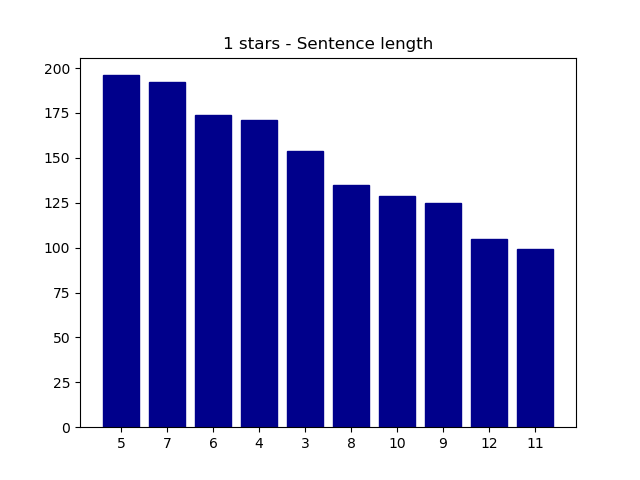
\includegraphics[scale=0.3]{figures/1stars-Sentencelength.png}
		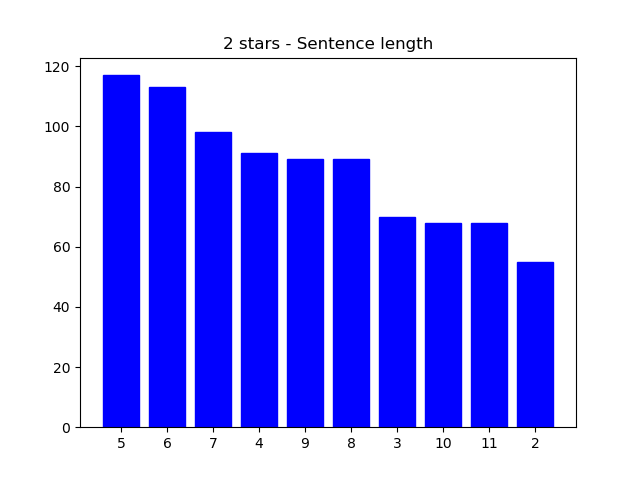
\includegraphics[scale=0.3]{figures/2stars-Sentencelength.png}
		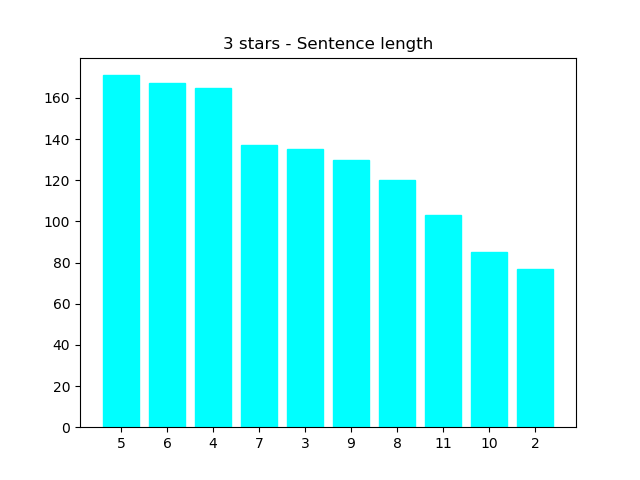
\includegraphics[scale=0.3]{figures/3stars-Sentencelength.png}
		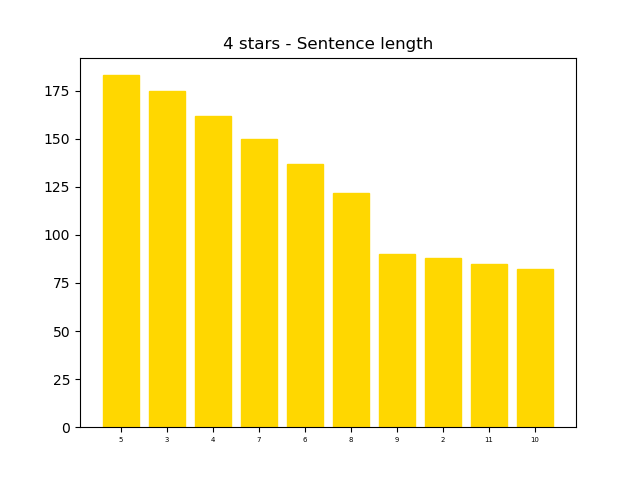
\includegraphics[scale=0.3]{figures/4stars-Sentencelength.png}
		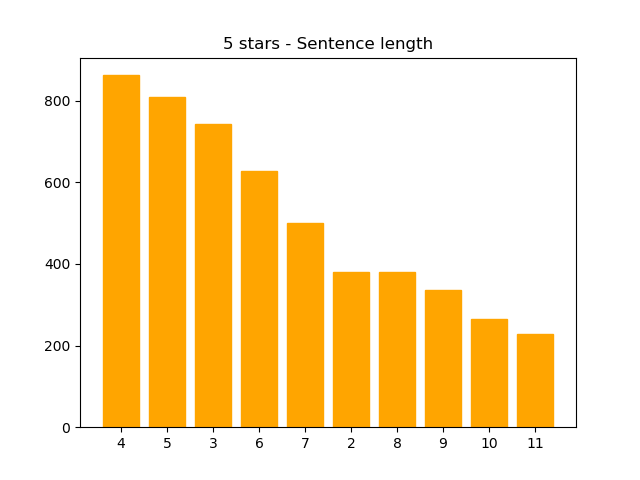
\includegraphics[scale=0.3]{figures/5stars-Sentencelength.png}
	\end{figure}
	As can be seen, the length of sentences is on average longer with a poor rating than with a good rating. 
	